\section{模型的建立与求解}

\subsection{数据预处理与审计}\label{sec:prep}

\textbf{数据审计发现（先于一切建模）}。逐表核对附件实际文件得到四个影响建模路线的事实：(i) A10/A11（1B 验证集）配比表 64 行、损失表 63 行，按 \texttt{index} 取交集使用；(ii) A16 的 17 域映射中仅 3 个 direct、3 个 near\_direct，11 个域无质量映射（inferred）；(iii) B1（Pythia 训练日志 1{,}176 行）可被三参数形式拟合至 $\mathrm{RMSE}=1.5\times10^{-4}$，呈公式生成特征；(iv) B8 与 B6/B7 在相同 $(N,D,Q)$ 点损失相关 $-0.03$ 且方向相反，两表不可比，B8 不参与联合拟合。

\textbf{指标展开}。22 个字段按输出形态展开为 25 个指标：二元 logits（\texttt{fluency\_en}、\texttt{ad\_en}）取 $\mathrm{softmax}$ 后正类概率；6 档 logits（\texttt{modernbert} 四字段）取期望档位 $\sum_k k\,\sigma_k/5$；\texttt{qurater} 拆为写作/专业/事实/教育四个独立维度；\texttt{fineweb\_edu} 直取；DSIR 三项为负对数比，仅域内可比；15 个规则统计量按定义方向处理。

\textbf{域内稳健归一}。每域每指标依次做：适宜区间型指标（词数、词长、一元熵等）以距域内中位数偏离改单峰；重尾指标先 $\log(1+x)$；$1\%/99\%$ 缩尾；域内 Min--Max 至 $[0,1]$；负向指标取补。全部变换参数在 A1 上估计后\textbf{冻结}，原样应用于 A2/A3——否则管线差异会混入抽样偏差，破坏对照的归因（这也是"同一管线"为题目强制的原因）。A1--A3 缺失率均低于 $0.03\%$，以域内中位数填补。

\subsection{问题一 (a)：综合质量评分}\label{sec:m1a}

\textbf{主线：CRITIC 客观赋权 + 加权几何平均。}指标 $j$ 的信息量与权重为
\begin{equation}
C_j=\sigma_j\sum_{k=1}^{25}\bigl(1-r_{jk}\bigr),\qquad
w_j=C_j\Big/\sum_k C_k,\qquad
Q(x)=\prod_{j=1}^{25} z_j(x)^{\,w_j},
\label{eq:critic}
\end{equation}
其中 $\sigma_j$ 为对比强度、$r_{jk}$ 为指标相关。选 CRITIC 而非熵权，是因其额外惩罚冗余指标（如 \texttt{fluency} 与 \texttt{readability} 高相关时权重自动分摊）；选几何平均而非算术平均，是因乘法形式实现"短板支配"——广告概率经补转换趋零时总分被显著压低，与 FineWeb-Edu/DCLM 的一票否决式过滤实践的方向一致但保留连续性。

\textbf{对照方法组}。等权几何平均、PCA（取累计方差 $80.6\%$ 的 10 个主成分、按方差贡献率合成，载荷矩阵输出至附表）、TOPSIS（以 CRITIC 权重加权的理想解贴近度）、K-means 三档聚类（仅给"优/普通/劣"相对档位）。样本级排序一致性：CRITIC 对等权 Spearman $0.991$、对 TOPSIS $0.946$、对 PCA $0.871$——三套互不蕴含的赋权假设给出高度一致的排序，说明质量结构是数据内在的而非赋权人为制造；K-means 的档位边界与连续分的分位一致，但聚类无法输出问题三成本函数所需的连续 $Q$，故仅作佐证。

\textbf{域级聚合与抽样代表性}。域级分取中位数主口径并报 token 加权副口径与 bootstrap 95\% CI（$B{=}2000$）。七域排序：arxiv $0.713>$ stackexchange $0.590>$ commoncrawl $0.557>$ github $0.533>$ book $0.511>$ c4 $0.499>$ wikipedia $0.484$（图~\ref{fig:box}）。以同一冻结管线复算 A2（arxiv 全量 17{,}523 篇）与 A3（github 全量 203{,}752 篇）：与 A1 对应子集的 KS 检验 $D=0.021\ (p=0.60)$ 与 $D=0.012\ (p=0.12)$，Cohen's $d\approx0.005$——抽样集代表性良好，域级结论可由抽样外推。

\begin{figure}[H]
\centering
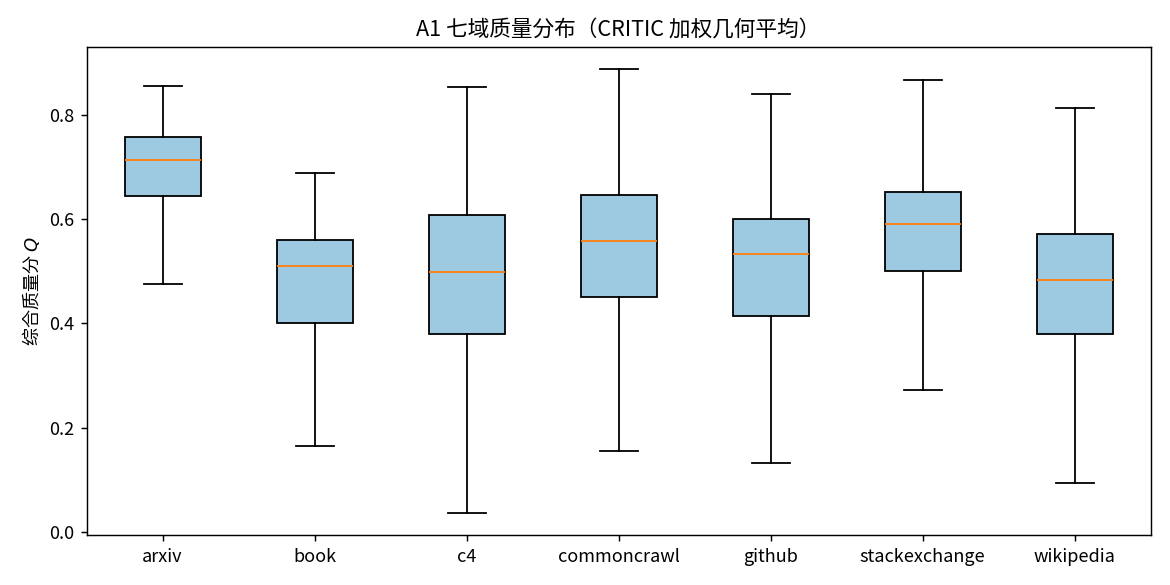
\includegraphics[width=.72\textwidth]{F2_domain_quality_box.png}
\caption{A1 七域质量分布（CRITIC 加权几何平均）。arxiv 显著最高；book 域仅 171 篇，其区间最宽。}
\label{fig:box}
\end{figure}

\subsection{问题一 (b)：指标冲突的定义、成因与消解}\label{sec:m1b}

\textbf{冲突定义（拒绝预设阈值）}。25 指标按信号来源分四组（规则型/DSIR/轻量分类器/模型评分器），组内 Kendall $W$ 分别为 $0.128/0.998/0.627/0.447$——同源信号一致性高，冲突主要发生在跨组，故在组级定义冲突：组分数取组内指标中位数，再转域内分位排名 $R_g(x)\in[0,1]$，冲突度 $c(x)=\max_g R_g-\min_g R_g$。阈值 $\tau$ 由冲突率—阈值曲线的最大曲率点确定（图~\ref{fig:conf}），得 $\tau=0.75$。

\textbf{测得冲突率 $21.5\%$}，直接否定《数据说明》页眉"冲突率约 $0\%$"的说法——后者以预设小阈值定义冲突再宣布无冲突，属把结论藏进定义。冲突与域强相关（$\chi^2=142.4$，$\mathrm{df}=6$，$p\approx10^{-23}$）；主冲突类型为"DSIR 高 $\times$ 规则型低"，在 A1/A2/A3 中占比 $19.6\%/15.1\%/18.1\%$，跨集复现；扩展集冲突率 $21.1\%$（A2）与 $22.9\%$（A3），与抽样集一致。对 30 篇高冲突文档的原文抽查（A1 含 \texttt{content}）证实两类机制：LaTeX/代码文本的专业价值高而表层流畅度指标低；模板化网页的规则统计量佳而模型评分器判为低教育价值。

\textbf{消解：Huber 连续降权}。对文档 $x$ 的组 $g$，按其排名偏离文档自身中位排名的程度 $\mathrm{dev}_g$ 施加权重 $u_g=\min(1,\tau_z/|\mathrm{dev}_g|)$，与 CRITIC 权重逐指标相乘后重归一，重算式~\eqref{eq:critic} 得修正分 $\widetilde Q$。效果：保序（$\rho(Q,\widetilde Q)=0.997$），冲突样本平均下调 $0.0033$ 而非冲突样本几乎不动（$-0.0004$）——降权而非删除，保留矛盾信息且不误伤专业语料；这是相对工业界硬过滤的改进点。严格口径的对照（冲突文档组分数取调和平均，下调 $0.149$）供敏感性使用。

\begin{figure}[H]
\centering
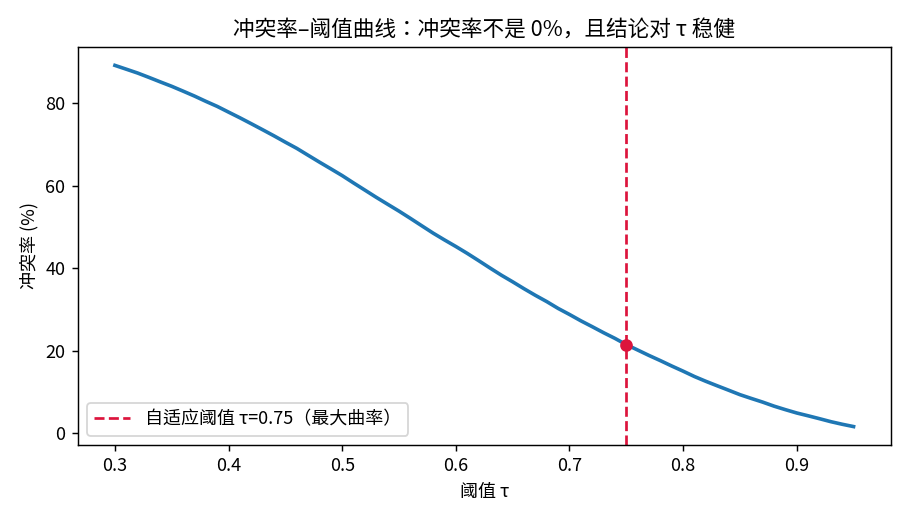
\includegraphics[width=.6\textwidth]{F3_conflict_rate_curve.png}
\caption{冲突率—阈值曲线与最大曲率点。结论在 $\tau\in[0.6,0.85]$ 内定性不变。}
\label{fig:conf}
\end{figure}

\subsection{跨体系桥接：17 个配比域的质量分}\label{sec:m1bridge}

11 个 inferred 域无官方质量信号。利用规则统计量\emph{可精确复算}的性质补全：自实现 11 个 \texttt{rps} 规则算子 $\Phi(\text{text})$，在 A1 上（每篇同时具备 $\Phi$ 与 $\widetilde Q$，$n=21{,}590$）以域分层五折交叉验证训练校准函数 $\hat g:\Phi\mapsto\widetilde Q$（梯度提升，$R^2_{\mathrm{cv}}=0.31$，优于岭回归 $0.25$）；再对 A18 的 17 域原文（31{,}340 篇）计算 $\hat Q=\hat g(\Phi)$ 并域级聚合。6 个有映射域上校准分与官方分互验：Pearson $0.70$、MAE $0.055$。最终 $\hat Q_d$ 取"映射域用官方分、inferred 域用校准分"，全部带 bootstrap CI 与证据等级标注（图~\ref{fig:bridge}）：最高 arxiv $0.716$，最低 dm\_mathematics $0.355$；ubuntu\_irc（16 篇）与 philpapers（63 篇）标注低置信。

\begin{figure}[H]
\centering
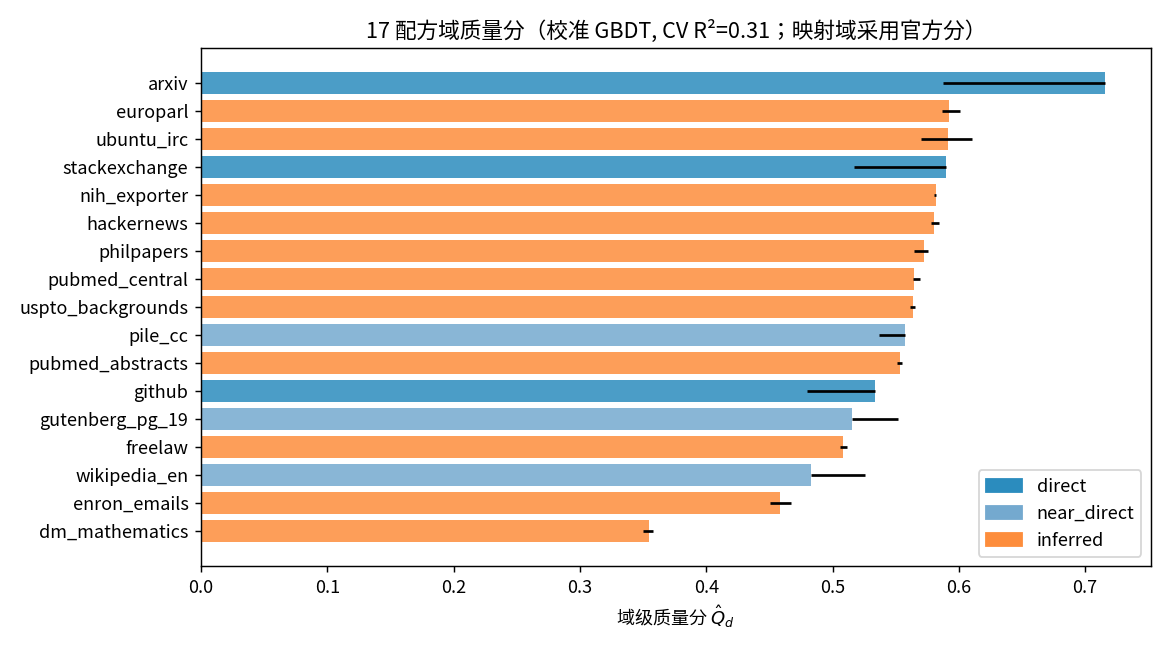
\includegraphics[width=.8\textwidth]{F4_bridge_17domains.png}
\caption{17 配比域质量分（颜色为映射类型；误差条为 bootstrap 95\% CI）。}
\label{fig:bridge}
\end{figure}

\subsection{问题一 (c)：配比—损失建模与最优配比}\label{sec:m1c}

\textbf{clr 变换消闭合效应（改进点）}。配比是成分数据：某域份额上升必然伴随其余域合计下降，直接回归会把机械的"此消彼长"误读为领域替代关系（Aitchison, 1986）。对 $\bm p$ 做中心对数比变换 $z_i=\ln(p_i/g(\bm p))$（$g$ 为几何均值，零分量乘性替换 $10^{-4}$），对每个验证域在对数空间回归：
\begin{equation}
\ln L_v=b_v+\sum_{i=1}^{17}\beta_{v,i}\,z_i+\varepsilon_v,
\qquad v=1,\dots,13,
\label{eq:clr}
\end{equation}
以 Huber 损失抗异常配方。1M 检验集（256 组）对照：\textbf{clr+Huber 的平均 $R^2=0.772$，裸配比 OLS（RegMix 原式）仅 $0.654$}（RMSE $0.320$ vs $0.432$）——闭合效应处理的收益即本方案对文献的量化改进。梯度提升作非线性对照（$R^2=0.897$），表明存在域间交互；故\emph{系数解释用线性、最优搜索用非线性}，两者在 $10^5$ 个候选配比上的目标损失秩相关 $0.77$，互为校验。

\textbf{迁移矩阵}。式~\eqref{eq:clr} 系数经链式法则折算到单纯形切空间，得 $T_{iv}=\partial\ln L_v/\partial p_i$（均匀配比处，图~\ref{fig:tm}）。全部 13 个自域效应为负（增配本域降本域损失），dm\_mathematics 自域效应最强（$-2.47$）；跨域外溢揭示 stackexchange 与 github 的互补结构。四个无损失列的域（nih\_exporter 等）保留为解释变量，其效应经由相对配比间接体现。

\begin{figure}[H]
\centering
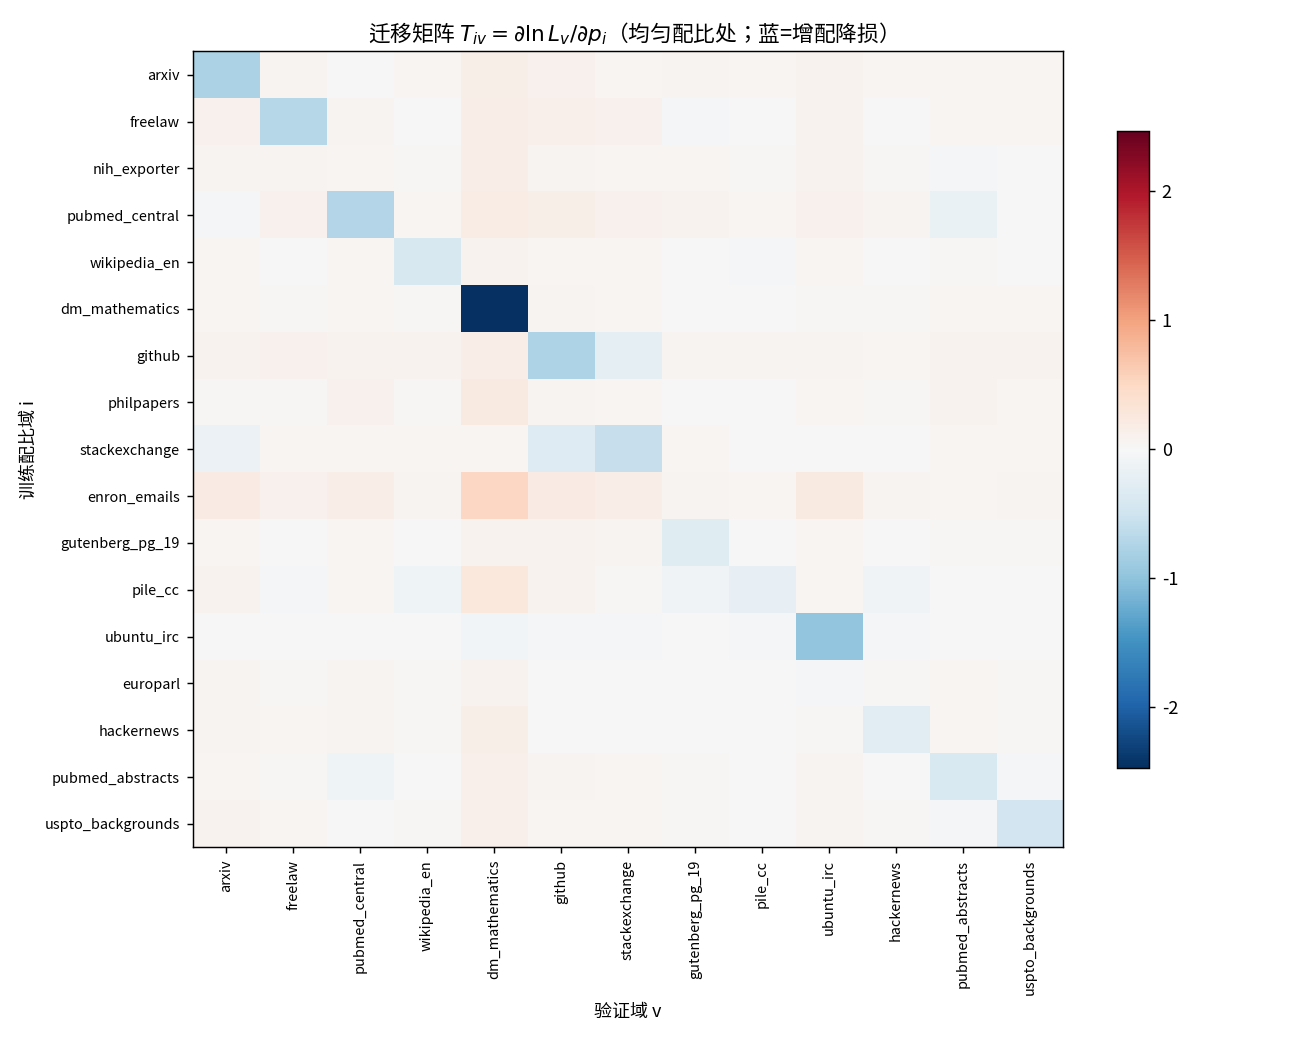
\includegraphics[width=.8\textwidth]{F5_transfer_matrix.png}
\caption{迁移矩阵 $T_{iv}$：蓝色为增配降损。对角占优，含非对角互补结构。}
\label{fig:tm}
\end{figure}

\textbf{质量交互项检验}。在式~\eqref{eq:clr} 加入 $\lambda_v\sum_ip_i(1-\hat Q_{d(i)})$ 作嵌套检验：$10/13$ 个验证域 $\lambda_v$ 显著（bootstrap 95\% CI 不含零）且加项后检验集 RMSE 全部不升；但\textbf{符号域间不一致}（中位数 $-0.249$，arxiv 域 $+0.79$）。结论：质量对配比—损失关系有独立解释力，但作用方向依验证域条件化——这提示问题二不应把质量与配比合并为单一乘子，二者应分开进入广义律。

\textbf{最优配比}。以训练配比均值为中心的多浓度 Dirichlet 采样 $10^5$ 个候选，取预测目标损失最优的前 100 个平均：等权口径 $\bm p^*$ 前五位为 pile\_cc $15.6\%$、stackexchange $10.0\%$、wikipedia $9.5\%$、pubmed\_central $9.1\%$、arxiv $8.9\%$；相对均匀配比预测降损 $9.9\%$（固定 $\bm p^*$ 的 bootstrap 95\% CI $[9.7\%,14.1\%]$）。pile\_cc 单域口径下 pile\_cc 占 $33.2\%$，复现 RegMix"网页语料对下游最有利"的反直觉结论。

\textbf{跨尺度验证与外推（假设~\ref{asm:proxy} 的检验）}。1M 系数直接预测三尺度留出集的目标损失排名：Spearman $0.52$（1M 留出）$/0.47$（60M）$/0.68$（1B）——排序中等保持；但 60M/1B 的绝对预测完全失效（$R^2$ 为大负值），系数漂移分解显示\textbf{截距显著下漂而斜率几乎不漂}（$\max_i|\rho_{\beta}|\approx0.007$）：配比效应结构稳定，基线水平随规模下移。对 A12--A15（10B/70B，幂律外推生成、非观测）：直接套 1M 系数 MAE $\approx3.5$ 完全不可用，以三尺度估计的漂移律 $b_v(N)=b_v^0+\rho_v\ln(N/10^6)$ 修正后 MAE 收窄至 $0.10$（35 倍改善）。外推稳健域排序：arxiv/pubmed\_central 最稳（$\rho>0.85$），pile\_cc/pubmed\_abstracts 最不稳（$\rho<0.40$）。

\textbf{质量 $\ne$ 训练价值}。域级质量分 $\hat Q_d$ 与训练边际价值 $\nu_d=-(\bar\beta_d-\overline{\bar\beta})$ 的秩相关 $\rho_{Q\nu}=-0.06$（图~\ref{fig:qv}）：内在质量几乎不预测训练价值，配比必须由实验回归而非质量排名确定。该结论直接支撑问题二将 $Q$ 与 $\bm p$ 设为两个独立自变量。

\begin{figure}[H]
\centering
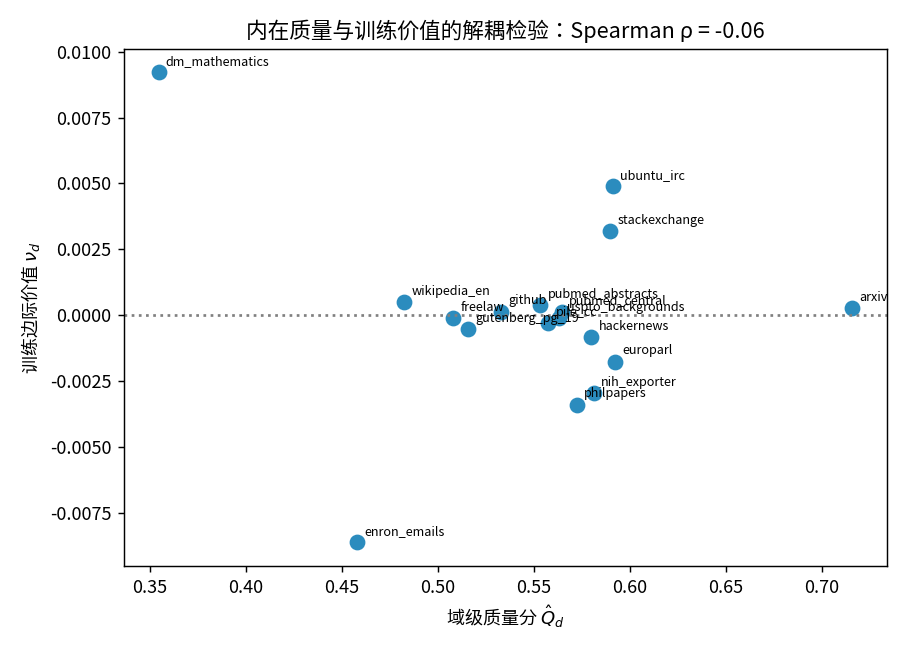
\includegraphics[width=.62\textwidth]{F7_quality_vs_value.png}
\caption{质量—价值解耦：dm\_mathematics 质量最低却训练边际价值最高。}
\label{fig:qv}
\end{figure}

\subsection{问题二：广义标度律的形式选择与拟合}\label{sec:m2fit}

\textbf{两步拟合}。第一步在 B1 上网格搜索 $(\alpha,\beta)$ 并最小二乘定 $(E,A,B)$，得 $L_0=1.6901+406.4N^{-0.340}+410.6D^{-0.280}$（$\mathrm{RMSE}=1.5\times10^{-4}$；该表呈公式生成特征，故此步为无噪声锚定）。第二步固定基线，在 B7（450 点）上对嵌套族做五折交叉验证：

\begin{table}[H]
\centering\small
\caption{质量项形式选择（cv-RMSE；数据噪声水平 $\sigma\approx0.05$）}
\begin{tabular}{lcc}
\toprule
候选形式 & cv-RMSE & 备注 \\
\midrule
耦合 + 地板（主） $\;h_N,h_D,k_0$ & $\bm{0.0497}$ & \textbf{主模型}（达噪声下限） \\
旧加性 $\;(1-Q)(k_0+k_1N^{-\alpha})$ & $0.0512$ & $\kappa_D=0$ 特例 \\
有效数据 $\;\kappa_N=0$ & $0.0979$ & 文献口径，单参数中最差 \\
\bottomrule
\end{tabular}
\label{tab:forms}
\end{table}

文献偏好的"质量折算有效数据量"乘子族（Muennighoff 风格）在本题数据上系统性落败——\emph{模型形式由交叉验证裁决而非先验借用}。主模型为

\begin{equation}
\boxed{\;L=\bigl\{E+A N^{-\alpha}h_N(Q)+B D^{-\beta}h_D(Q)+k_0(1-Q)\bigr\}\,e^{s(N)[\bar f(\bm p)-\bar f(\bm p^*)]}\;}
\label{eq:main}
\end{equation}

\begin{table}[H]
\centering\small
\caption{广义标度律参数（残差 bootstrap $B=300$）}
\begin{tabular}{cccccccc}
\toprule
$E$ & $A$ & $\alpha$ & $B$ & $\beta$ & $\kappa_N$ & $\kappa_D$ & $k_0$ \\
\midrule
$1.6901$ & $406.4$ & $0.340$ & $410.6$ & $0.280$ &
$\underset{[0.390,\,0.473]}{0.431}$ & $\underset{[0.085,\,0.195]}{0.140}$ &
$\underset{[0.114,\,0.168]}{0.141}$ \\
\bottomrule
\end{tabular}
\label{tab:params}
\end{table}

其中 $h_N=1+\kappa_N(1-Q)$，$h_D=1+\kappa_D(1-Q)$，$s(N)=\max\{1.003-0.077\log_{10}(N/10^6),0\}$。$Q=1$ 且 $\bm p=\bm p^*$ 时式~\eqref{eq:main} 退化为经典 Chinchilla 形式。主口径 $Q_{\mathrm B}=\bar q(\bm p)$，$Q_0=0.6609$。配比经问题一接口引入，不重复读取附件 A；域结构效应由迁移矩阵 $T$ 单独描述。

\textbf{跨源检验}。真实文献点上主模型预测与观测的 Spearman：scaling\_baseline（57 点）$0.983$、published（44 点）$0.959$，平均偏差 $0.22/0.02$ nats——趋势一致，绝对偏移源于 tokenizer 与验证集差异，符合"跨源只比趋势"的审计原则；B2（Cerebras 半合成）偏差 $1.18$ nats，仅作定性佐证。

\subsection{问题二：解析理论}\label{sec:m2theory}

以下命题由式~\eqref{eq:main} 直接推导，全部与数值优化互验（相对误差 $<10^{-6}$）。

\begin{proposition}[弹性]\label{prop:el}
记 $\Phi=\kappa_N AN^{-\alpha}+\kappa_D BD^{-\beta}+k_0$，则
$\displaystyle
\varepsilon_N=-\frac{\alpha A N^{-\alpha}h_N}{L},\quad
\varepsilon_D=-\frac{\beta B D^{-\beta}h_D}{L},\quad
\varepsilon_Q=-\frac{Q\,\Phi}{L}.$
在 $(N,D,Q)=(10^{10},10^{12},0.9)$ 处三者为 $-0.028/-0.025/-0.103$：\emph{质量弹性约为参数弹性的 $3.7$ 倍}。
\end{proposition}

\begin{proposition}[质量—参数等效替代及其边界]\label{prop:sub}
固定 $D$，使 $L(N',D,Q)=L(N,D,Q+\delta)$ 的等效参数量
\begin{equation}
\frac{N'}{N}=t^{-1/\alpha},\quad
t=\frac{h_N(Q+\delta)}{h_N(Q)}-\frac{\delta(\kappa_D BD^{-\beta}+k_0)}{AN^{-\alpha}h_N(Q)},
\end{equation}
当且仅当 $t>0$ 时有限。算力最优点上 $Q_{\mathrm B}:0.5\to0.6$ 等效参数 $1.29/1.42/1.77$ 倍（$C=10^{20}/10^{22}/10^{24}$）。同一份质量改进，模型越大越值钱。
\end{proposition}

\begin{proposition}[质量地板]\label{prop:fl}
$\lim_{N,D\to\infty}L=E+(1-Q)k_0$。$Q=0.5$ 的地板比 $Q=1$ 高 $0.070$ nats。该地板是 B6/B7 的生成特征，外推须标注。
\end{proposition}

\begin{proposition}[算力最优配置随质量移动]\label{prop:opt}
约束 $6ND=C$ 下，
\begin{equation}
N^{*}(C,Q)=\Bigl[\frac{\alpha A\,h_N(Q)}{\beta B\,h_D(Q)}\Bigr]^{\frac{1}{\alpha+\beta}}
\Bigl(\frac{C}{6}\Bigr)^{\frac{\beta}{\alpha+\beta}},\qquad \frac{\beta}{\alpha+\beta}=0.452.
\end{equation}
因为 $\kappa_N>\kappa_D$，质量越低最优模型越大：$Q_{\mathrm B}=0.3$ 时的 $N^*$ 是 $Q_{\mathrm B}=1$ 时的 $1.32$ 倍。$C=10^{22}$ 时最优 token/参数比从 $Q=0.3$ 的 36 升至 $Q=1$ 的 63。
\end{proposition}

\begin{figure}[H]
\centering
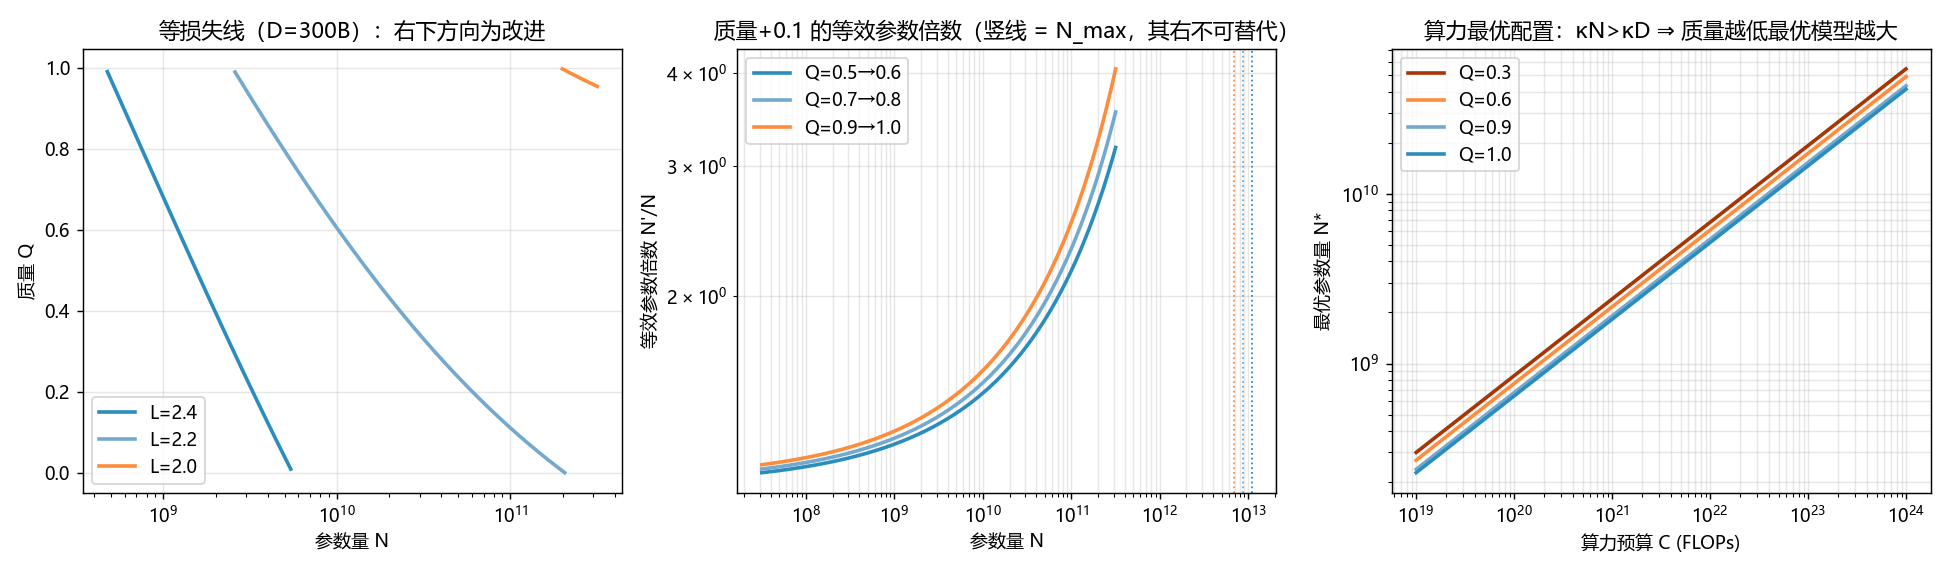
\includegraphics[width=\textwidth]{F21_theory.png}
\caption{解析理论三联图：等损失线（左）、等效参数倍数（中）、$N^*(C,Q)$（右）。}
\label{fig:theory}
\end{figure}
